%%%%%%%%%%%%%%%%%%%%%%%%%%%%%%%%%%%%%%%%%%%%%%%%%%%%%%%%%%%%%%%%%%%%%%%%%%%%%%%%
%2345678901234567890123456789012345678901234567890123456789012345678901234567890
%        1         2         3         4         5         6         7         8

\documentclass[letterpaper, 10 pt, conference]{ieeeconf}

\IEEEoverridecommandlockouts
\overrideIEEEmargins

\usepackage{cite}
\usepackage{amsmath,amssymb,amsfonts}
\usepackage{algorithmic}
\usepackage{graphicx}
\usepackage{textcomp}
\usepackage{xcolor}
\usepackage{float}
\usepackage{multirow}
\usepackage[utf8]{inputenc}
\usepackage[T1]{fontenc}
\usepackage[brazil]{babel}

\graphicspath{{../IJCNN/}}

\def\BibTeX{{\rm B\kern-.05em{\sc i\kern-.025em b}\kern-.08em
    T\kern-.1667em\lower.7ex\hbox{E}\kern-.125emX}}

% -----------------------------------------------------------------------

\title{\LARGE \bf
Análise por Camada e Fusão Adaptativa com Mixture of Experts em Modelos
Profundos para Classificação de Cor e Textura
}

\author{
    Arlete T. Beuren\textsuperscript{1},
    Vinícius C. Ribeiro\textsuperscript{1},
    Leonardo J. R. Pinto\textsuperscript{1},
    Jonathan de Matos\textsuperscript{2},
    Alceu S. Britto Jr.\textsuperscript{2,3}%
    \thanks{Este trabalho foi apoiado pelo Conselho Nacional de
            Desenvolvimento Científico e Tecnológico (CNPq, Brasil).}%
    \thanks{\textsuperscript{1}Universidade Tecnológica Federal do Paraná
            (UTFPR), Santa Helena (PR), Brasil.
            \texttt{arletebeuren@utfpr.edu.br}}%
    \thanks{\textsuperscript{2}Universidade Estadual de Ponta Grossa (UEPG),
            Ponta Grossa (PR), Brasil.
            \texttt{jonathan@uepg.br}}%
    \thanks{\textsuperscript{3}Pontifícia Universidade Católica do Paraná
            (PUCPR), Curitiba (PR), Brasil.
            \texttt{alceu@ppgia.pucpr.br}}%
}

% -----------------------------------------------------------------------

\begin{document}

\maketitle
\thispagestyle{empty}
\pagestyle{empty}

% -----------------------------------------------------------------------
\begin{abstract}

Este trabalho investiga a sensibilidade por camada de modelos profundos
para a classificação de atributos visuais de cor e textura, e propõe uma
estratégia de fusão adaptativa baseada em Mixture of Experts~(MoE).
Experimentos são conduzidos com cinco arquiteturas — ResNet-50, VGG-16,
iBOT, VMamba e LMFCN — sobre um conjunto de dados de moda com 1.000
imagens de cor e 1.000 de textura.
O \emph{Experimento~1} confirma que camadas rasas são mais eficazes para
cor, enquanto camadas profundas capturam melhor textura, padrão que se
generaliza de CNNs clássicas a Transformers de Visão e Modelos de Espaço
de Estados.
O \emph{Experimento~2} mostra que a concatenação simples de camadas rasa e
profunda geralmente não supera representações especializadas de camada única.
O \emph{Experimento~3} introduz um modelo MoE treinável que, por meio de um
roteador aprendido, pondera adaptativamente as contribuições da camada rasa
(cor) e da camada profunda (textura) por imagem.
O MoE supera tanto o Experimento~1 quanto o Experimento~2 em quase todas as
arquiteturas, alcançando até 98,00\% com VMamba em textura e 97,33\% com
iBOT em cor — melhorias de 2,24 e 1,46 pontos percentuais sobre as melhores
camadas individuais, respectivamente.

\end{abstract}

\begin{IEEEkeywords}
Redes Neurais Convolucionais, Modelos Profundos, Atributos Visuais,
Vision Transformers, Modelos de Espaço de Estados, Mixture of Experts,
Recuperação de Imagens.
\end{IEEEkeywords}

% -----------------------------------------------------------------------
\section{INTRODUÇÃO}

Os avanços em redes neurais convolucionais~(CNNs) viabilizaram soluções cada
vez mais eficazes em visão computacional para aplicações industriais.
Um exemplo proeminente é a recuperação de imagens em comércio eletrônico,
onde consultas podem ser realizadas por texto, imagem ou combinações
multimodais~\cite{b1}.

Sistemas de recuperação baseada em conteúdo~(CBIR) apresentam desafios
únicos e possuem aplicações em imagens médicas, sistemas de informação
geográfica e vigilância~\cite{b12}.
Um desafio central consiste em extrair com precisão atributos visuais
relevantes, especialmente quando a consulta do usuário é guiada por
propriedades específicas como cor, textura ou sua combinação
(Figura~\ref{fig_patterns}).

\begin{figure}[htbp]
\centerline{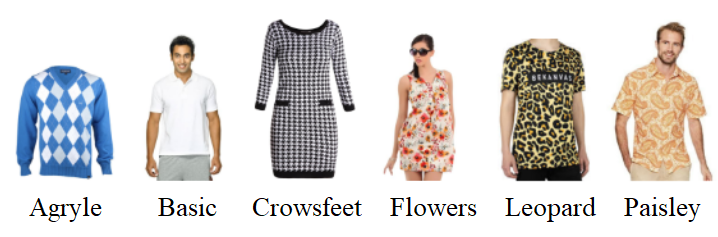
\includegraphics[width=0.48\textwidth]{fig_texture_samples.png}}
\caption{Seis padrões distintos baseados em cor e textura
         (adaptado de~\cite{b2}).}
\label{fig_patterns}
\end{figure}

A extração de características de cor e textura é tema central em CBIR.
Descritores clássicos incluem histogramas de cor e momentos de cor, que
capturam propriedades estatísticas como média, variância e assimetria das
distribuições de cor~\cite{b24}.
Para textura, filtros de Gabor e Padrões Binários Locais~(LBP) têm sido
amplamente utilizados~\cite{b25}.

Com o advento do aprendizado profundo, Baloian et al.~\cite{b2}
demonstraram que camadas distintas de CNNs exibem sensibilidade específica
a atributos, com camadas iniciais mais sensíveis a cor e camadas profundas
capturando melhor textura.
Contudo, o comportamento de representações por atributo em arquiteturas
modernas — Vision Transformers e Modelos de Espaço de Estados — permanece
pouco explorado, e estratégias de fusão adaptativa entre camadas
especializadas ainda são escassas na literatura.

Neste trabalho, avaliamos e comparamos arquiteturas clássicas e modernas
para classificação baseada em cor e textura.
Analisamos representações por camada para investigar a sensibilidade a
atributos visuais e a eficácia de diferentes estratégias de fusão.
Como contribuição principal, propomos um modelo de fusão adaptativa baseado
em Mixture of Experts~(MoE) que aprende, por imagem, os pesos relativos da
camada rasa~(cor) e da camada profunda~(textura) por meio de um roteador
treinável.

O conjunto de dados utilizado foi introduzido em~\cite{b2} e é composto
por imagens de moda coletadas do Kaggle e repositórios online, incluindo
chapéus, vestidos, camisas, meias, bolsas e lenços.
O conjunto é dividido em dois subconjuntos:
\begin{itemize}
  \item \textbf{Conjunto de cor}: 1.000 imagens em 10 classes de cor
        (vermelho, preto, azul, verde, amarelo, cinza, marrom, rosa, roxo e
        laranja), ilustrado na Figura~\ref{fig_color_samples};
  \item \textbf{Conjunto de textura}: 1.000 imagens em 10 classes de padrão
        de textura (xadrez, listrado, flores, leopardo, bolinhas, liso,
        paisley, losango, pé-de-galinha e paetê).
\end{itemize}

\begin{figure}[htbp]
\centerline{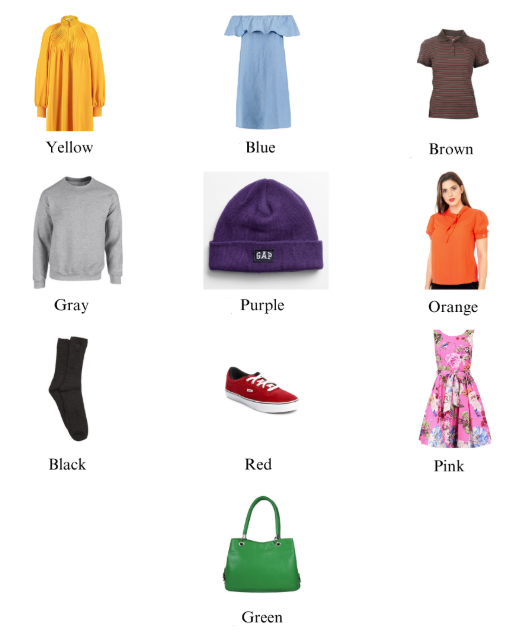
\includegraphics[width=0.48\textwidth]{fig_color_samples.png}}
\caption{Amostras de cada classe no conjunto de dados de cor.}
\label{fig_color_samples}
\end{figure}

As principais contribuições deste trabalho são:
\begin{itemize}
  \item Análise abrangente por camada da sensibilidade a atributos em CNNs
        clássicas, Vision Transformers e Modelos de Espaço de Estados;
  \item Benchmark comparativo de VGG-16, ResNet-50, iBOT, VMamba e LMFCN
        para classificação baseada em cor e textura;
  \item Demonstração experimental de que a fusão por concatenação simples
        não melhora o desempenho em tarefas de atributo específico;
  \item Proposta e avaliação de um modelo MoE que realiza fusão adaptativa
        de características rasa e profunda, superando concatenação e
        frequentemente superando camadas individuais especializadas.
\end{itemize}

Este artigo está organizado da seguinte forma.
A Seção~II apresenta trabalhos relacionados.
A Seção~III descreve as arquiteturas avaliadas.
A Seção~IV detalha a metodologia experimental.
A Seção~V apresenta os resultados.
A Seção~VI discute os achados e a Seção~VII conclui o trabalho.

% -----------------------------------------------------------------------
\section{TRABALHOS RELACIONADOS}

O uso de CNNs para representar similaridade entre objetos foi amplamente
explorado na literatura.
Baloian et al.~\cite{b2} investigaram o comportamento das camadas da
ResNet-50 para recuperação baseada em cor e textura, demonstrando que
camadas convolucionais iniciais são mais sensíveis à cor, enquanto camadas
mais profundas capturam melhor os padrões de textura.
Em seu framework, características foram extraídas da ResNet-50
pré-treinada no ImageNet~\cite{b3}, com \emph{Global Average Pooling}~(GAP)
aplicado a cada bloco residual e k-vizinhos mais próximos~(kNN) utilizado
para classificação com 5 repetições de holdout estratificado 70/30.

Estudos de aprendizado de representação para reconhecimento de objetos e
atributos incluem o trabalho de Liang et al.~\cite{b10}, que empregaram
redes neurais para aprender características discriminativas baseadas em
categorias de objetos, e Gan et al.~\cite{b11}, que propuseram técnicas de
generalização para domínio multi-fonte em aprendizado de atributos.
Arquiteturas siamesas foram investigadas para classificação de granularidade
fina; Moresco et al.~\cite{b8} demonstraram que a combinação de
características de camadas intermediárias melhora a classificação de
espécies de plantas, destacando a natureza complementar de representações
multi-camada.

Descritores clássicos de textura e cor permanecem relevantes.
Irtaza et al.~\cite{b13} propuseram um framework de extração de textura
baseado em pacotes wavelet e autovalores de filtros de Gabor combinados com
kNN parcialmente supervisionado.
Lin et al.~\cite{b15} introduziram vários descritores, incluindo matrizes de
co-ocorrência de cor~(CCM), diferença entre pixels~(DBPSP) e agrupamento
baseado em histograma de cor~(CHKM).

A fusão de características de múltiplas camadas foi proposta para combinar
representações de diferentes profundidades da rede.
Estratégias incluem fusão antecipada~(\emph{early fusion} por
concatenação de características), fusão tardia~(\emph{late fusion} em
nível de decisão) e fusão aprendida com mecanismos de atenção~\cite{b26,b27}.
No entanto, a eficácia dessas abordagens para tarefas de atributo específico
ainda é insuficientemente estudada.

Avanços recentes desafiaram a dominância de modelos baseados em
Transformer.
A arquitetura Mamba~\cite{b16}, um Modelo de Espaço de Estados Estruturado~(SSM),
alcança complexidade linear no comprimento da sequência, contra a
complexidade quadrática dos Transformers.
No domínio de visão autossupervisionada, o framework
iBOT~\cite{b17} introduziu um objetivo de modelagem de imagem mascarada com
tokenizador online, permitindo o aprendizado simultâneo de tokens visuais
discretos e representações semânticas.
O framework LMFCN~\cite{b28} propõe treinar redes totalmente
convolucionais~(FCNs) cujas representações são otimizadas para
classificação de grande margem com Máquinas de Vetores de Suporte~(SVMs).

A natureza hierárquica das representações em redes profundas foi
investigada desde os trabalhos seminais de Zeiler e Fergus~\cite{bzeiler},
que mostraram visualmente que camadas iniciais de CNNs respondem a bordas
e cores enquanto camadas profundas codificam padrões estruturais complexos.
Análises análogas para Vision Transformers foram conduzidas por
Kazami et al.~\cite{bkazami}, revelando que os blocos iniciais do ViT
preservam informação espacial de baixo nível e os blocos finais capturam
semântica global.
Em contraste com esses trabalhos, que realizam análise qualitativa ou de
visualização, o presente trabalho conduz uma avaliação quantitativa
sistemática de sensibilidade a atributos específicos~(cor e textura) por
camada, estendendo a análise a arquiteturas de Espaço de Estados~(VMamba)
ainda não contempladas na literatura de análise por camada, e propõe um
mecanismo de fusão adaptativa treinável baseado nessas observações.

A técnica de Mixture of Experts~(MoE) foi originalmente proposta por
Jacobs et al.~\cite{bmoe_orig} como uma arquitetura modular em que um
roteador aprende a dividir o espaço de entrada entre especialistas locais.
Trabalhos recentes exploram MoE em fusão multimodal de imagens: Cao
et al.~\cite{bmoe_cao} propuseram o MoE-Fusion, que combina especialistas
locais e globais por meio de um roteador com portão multimodal para fusão
dinâmica de imagens.
No entanto, a aplicação de MoE na seleção adaptativa de camadas por
profundidade dentro de um único backbone para atributos visuais específicos
permanece inexplorada.
O presente trabalho preenche essa lacuna propondo um roteador treinável que
aprende, por imagem, quanto ponderar a representação da camada rasa~(cor)
versus a camada profunda~(textura).

% -----------------------------------------------------------------------
\section{ARQUITETURAS AVALIADAS}

Esta seção descreve as cinco arquiteturas backbone utilizadas nos
experimentos.

\subsection{ResNet-50}

A ResNet-50~\cite{b4} é uma CNN de 50 camadas que emprega aprendizado
residual via conexões de atalho baseadas em identidade.
Esse projeto possibilita a otimização de arquiteturas profundas ao
reformular o objetivo de aprendizado como funções residuais, mitigando a
degradação do gradiente.
No Experimento~1, características foram extraídas de cada bloco residual
via GAP (dimensões: 256, 512, 1024 e 2048).
No modelo MoE, a camada rasa corresponde ao Bloco Residual~1~(256d) e a
camada profunda ao Bloco Residual~3~(1024d)
(Figura~\ref{fig_resnet}).

\begin{figure}[htbp]
\centerline{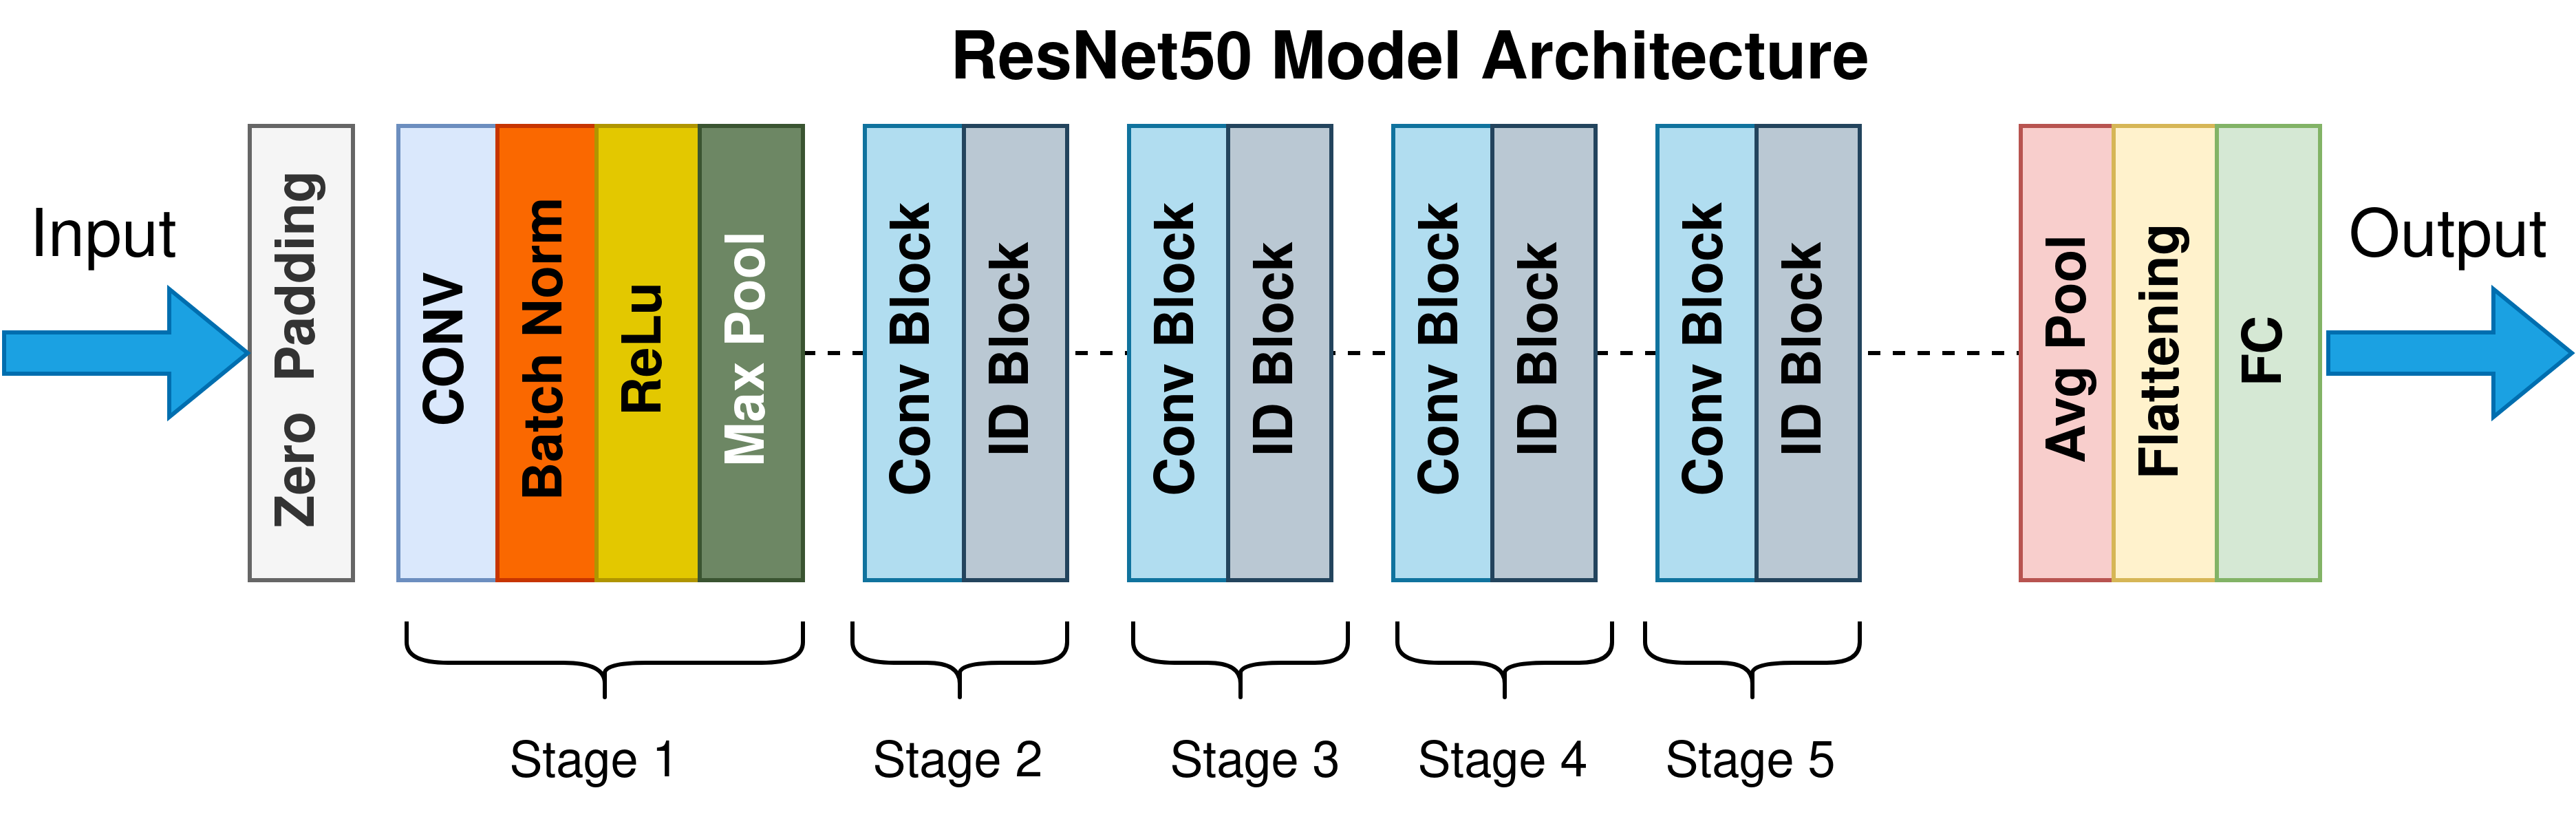
\includegraphics[width=0.48\textwidth]{resnet50.png}}
\caption{Arquitetura da ResNet-50. Adaptado de Mukherjee~\cite{b23},
         baseado em He et al.~\cite{b4}.}
\label{fig_resnet}
\end{figure}

\subsection{VGG-16}

A VGG-16~\cite{b7} emprega uma arquitetura homogênea com camadas
convolucionais $3 \times 3$ empilhadas, composta por 5 blocos convolucionais
com dimensões de saída 64, 128, 256, 512 e 512.
No modelo MoE, a camada rasa corresponde à saída do Bloco~1~(64d) e a camada
profunda à saída do Bloco~3~(256d)
(Figura~\ref{fig_vgg}).

\begin{figure}[htbp]
\centerline{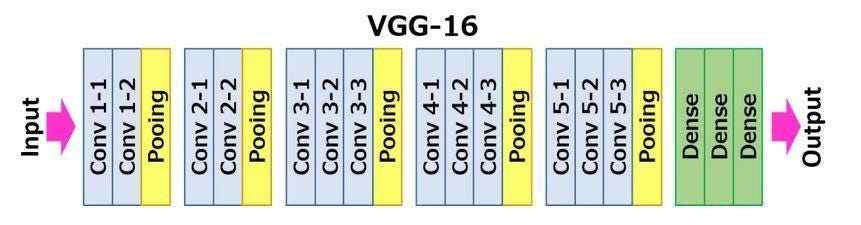
\includegraphics[width=0.48\textwidth]{VGG16.jpg}}
\caption{Arquitetura da VGG-16.
         Fonte: Simonyan \& Zisserman~\cite{b7}.}
\label{fig_vgg}
\end{figure}

\subsection{VMamba}

O VMamba~\cite{b16} representa uma nova classe de modelos de sequência
baseados em SSMs.
Ao contrário dos Transformers, que têm complexidade quadrática em relação
ao comprimento da sequência, o VMamba processa sequências em tempo linear
por meio de um mecanismo de varredura seletiva.
Utilizamos a variante VMamba-Tiny; características foram extraídas de cada
um de seus quatro estágios via GAP (dimensões: 96, 192, 384 e 768).
No MoE, a camada rasa é o Estágio~1~(192d) e a profunda é o
Estágio~2~(384d) (Figura~\ref{fig_mamba}).

\begin{figure}[htbp]
\centerline{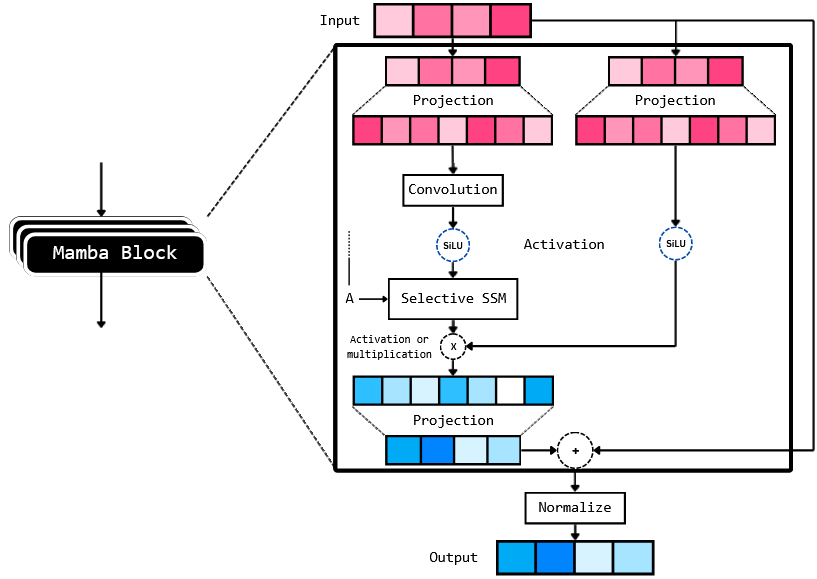
\includegraphics[width=0.48\textwidth]{Vmamba.png}}
\caption{Diagrama do bloco Mamba.
         Fonte: Gu \& Dao~\cite{b16}.}
\label{fig_mamba}
\end{figure}

\subsection{iBOT}

O iBOT~\cite{b17} é um framework autossupervisionado baseado em Vision
Transformers~(ViT) que utiliza modelagem de imagem mascarada com
tokenizador online.
Utilizamos o backbone ViT-S/16; características foram extraídas de cada
um dos 12 blocos transformer via token CLS (384~dimensões cada).
No MoE, a camada rasa é o Bloco~2 e a camada profunda é o Bloco~9
(Figura~\ref{fig_ibot}).

\begin{figure}[htbp]
\centerline{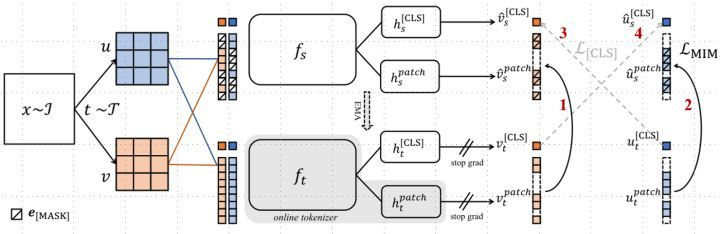
\includegraphics[width=0.48\textwidth]{Ibot.jpg}}
\caption{Visão geral do framework iBOT.
         Fonte: Zhou et al.~\cite{b17}.}
\label{fig_ibot}
\end{figure}

\subsection{LMFCN}

A LMFCN~\cite{b28} recebe imagens como entrada, extrai representações via
uma Rede Totalmente Convolucional~(FCN) e utiliza essas características para
construir a matriz de kernel de uma SVM.
Durante o treinamento, os parâmetros da FCN são atualizados para maximizar
a margem entre classes.
Avaliamos arquiteturas TCNN (com 3 a 6 camadas) treinadas do zero e
variantes da ResNet-18 pré-treinada com os blocos finais removidos
(Figura~\ref{fig_lmfcn}).

\begin{figure}[htbp]
\centerline{\includegraphics[width=0.48\textwidth]{CNNSV4.eps}}
\caption{Visão geral da LMFCN.
         Fonte: de Matos et al.~\cite{b28}.}
\label{fig_lmfcn}
\end{figure}

% -----------------------------------------------------------------------
\section{METODOLOGIA EXPERIMENTAL}

\subsection{Conjunto de Dados e Protocolo}

O conjunto de dados utilizado é o mesmo introduzido por~\cite{b2}.
Consiste em 10 classes de cor e 10 classes de textura, com 100 imagens por
classe, totalizando 1.000 imagens para cada tarefa.
Os dados foram divididos em 70\% para treinamento e 30\% para teste,
com 5 repetições de holdout estratificado.

A avaliação das características extraídas foi realizada com um classificador
k-vizinhos mais próximos~(kNN) com $k = 5$ e distância euclidiana, sob o
mesmo protocolo de holdout com 5 repetições.

\subsection{Sensibilidade por Camada — Extração de Camada Única}

Para cada arquitetura, foram extraídas características de cada camada ou
bloco de processamento individualmente.
CNNs usam GAP para produzir um vetor por camada; iBOT usa o token CLS;
VMamba usa GAP no mapa de características de cada estágio.
Para LMFCN, são avaliadas variantes TCNN (3 a 6 camadas) e ResNet-18
com 2 ou 4 blocos residuais.

\subsection{Fusão por Concatenação Rasa–Profunda}

Para cada backbone, as características da melhor camada para cor~(E) e da
melhor camada para textura~(D) foram concatenadas:
$z = [f_E \; ; \; f_D]$, e o vetor resultante foi avaliado com kNN.

\subsection{Fusão Adaptativa com Mixture of Experts}

O modelo MoE introduzido neste trabalho aprende, por imagem, pesos
adaptativos $\alpha$ e $\beta$ para a camada rasa e a camada profunda,
respectivamente.

\textbf{Arquitetura.} Para cada backbone, dois projetores
$h_E$ e $h_D$ — compostos por uma camada linear, LayerNorm e ReLU —
mapeiam as características de dimensões heterogêneas para um espaço
comum de dimensão $d = 256$.
Um roteador~(Router), baseado em MLP com duas camadas e Softmax, recebe a
concatenação $[h_E(f_E) ; h_D(f_D)]$ e produz os pesos $\alpha$ e $\beta$
com $\alpha + \beta = 1$.
O vetor final é:
\begin{equation}
    z = \alpha \cdot h_E(f_E) + \beta \cdot h_D(f_D).
    \label{eq:moe}
\end{equation}

O backbone permanece congelado durante o treinamento; apenas $h_E$, $h_D$
e o Router são atualizados.
Uma cabeça linear auxiliar supervisiona o treinamento com
\emph{cross-entropy loss}; após o treinamento, somente os embeddings~$z$
são utilizados na avaliação com kNN.

\textbf{Protocolo de treinamento.} Otimizador AdamW, $lr = 10^{-4}$,
\emph{weight decay} $= 10^{-5}$, CosineAnnealingLR com $T_{max} = 30$
épocas, \emph{batch size} 32, \emph{data augmentation} básico~(recorte
aleatório 224$\times$224 e flip horizontal) somente no treinamento.
Avaliação final: kNN com $k = 5$ e StandardScaler nos embeddings~$z$,
sob o mesmo protocolo de holdout 70/30 com 5 repetições.

A Tabela~\ref{tab_moe_config} resume as camadas selecionadas como rasa e
profunda para cada backbone no MoE.

\begin{table}[htbp]
\caption{Configuração das camadas rasa e profunda no modelo MoE.}
\begin{center}
\begin{tabular}{c|c|c|c|c}
\hline
\textbf{Backbone} & \textbf{Rasa (E)} & \textbf{Dim~E}
                  & \textbf{Profunda (D)} & \textbf{Dim~D} \\
\hline
VGG-16     & Bloco 1      & 64   & Bloco 3      & 256  \\
ResNet-50  & Bloco Res. 1 & 256  & Bloco Res. 3 & 1024 \\
iBOT       & Bloco 2      & 384  & Bloco 9      & 384  \\
VMamba     & Estágio 1    & 192  & Estágio 2    & 384  \\
\hline
\end{tabular}
\label{tab_moe_config}
\end{center}
\end{table}

% -----------------------------------------------------------------------
\section{RESULTADOS EXPERIMENTAIS}

\subsection{Sensibilidade por Camada — CNNs Clássicas}

A Tabela~\ref{tab2} apresenta a acurácia de classificação obtida pelas
camadas da VGG-16 e pelos blocos residuais da ResNet-50.
Os resultados revelam uma clara relação entre profundidade e sensibilidade
ao atributo.
Na VGG-16, a Camada~1 obteve a maior acurácia de cor~(95,13\%), com
desempenho decrescente nas camadas mais profundas até 55,07\% na Camada~5.
Contrariamente, a acurácia de textura melhorou com a profundidade, com
pico na Camada~4~(94,73\%).
A ResNet-50 exibiu comportamento similar: o Bloco Residual~2 obteve o
melhor resultado de cor~(95,87\%), enquanto o Bloco Residual~3 foi mais
eficaz para textura~(93,27\%).

\begin{table}[htbp]
\caption{Acurácia das camadas da VGG-16 e blocos residuais~(BR) da ResNet-50
         para classificação de cor e textura.}
\begin{center}
\begin{tabular}{c|c|c|c|c|c}
\hline
\textbf{Camada} & \textbf{Cor} & \textbf{Std} & \textbf{Textura}
                & \textbf{Std} & \textbf{Dim} \\
\hline
VGG-16 Cam. 1 & \textbf{95,13} & 0,81 & 70,73 & 2,25 & 64   \\
VGG-16 Cam. 2 & 90,27 & 1,27 & 86,60 & 1,57 & 128  \\
VGG-16 Cam. 3 & 85,47 & 2,33 & 93,20 & 1,48 & 256  \\
VGG-16 Cam. 4 & 71,80 & 2,55 & \textbf{94,73} & 0,74 & 512  \\
VGG-16 Cam. 5 & 55,07 & 2,64 & 89,40 & 1,64 & 512  \\
ResNet-50 BR1 & 95,47 & 0,78 & 83,40 & 1,36 & 256  \\
ResNet-50 BR2 & \textbf{95,87} & 0,50 & 90,67 & 1,65 & 512  \\
ResNet-50 BR3 & 88,27 & 1,12 & \textbf{93,27} & 0,25 & 1024 \\
ResNet-50 BR4 & 59,20 & 3,11 & 86,33 & 0,92 & 2048 \\
\hline
\end{tabular}
\label{tab2}
\end{center}
\end{table}

\subsection{Sensibilidade por Camada — LMFCN}

A Tabela~\ref{tab1} apresenta os resultados da LMFCN.
No conjunto de textura, o aumento de profundidade da TCNN levou à melhoria
consistente de desempenho.
No conjunto de cor, acurácias mais altas foram obtidas nas camadas iniciais.
A LMFCN com SVM alcançou 96,87\%$\pm$0,9 em textura~(ResNet-18 com 2 blocos)
e 97,73\%$\pm$0,95 em cor~(TCNN3).

\begin{table}[htbp]
\caption{Acurácia dos blocos convolucionais~(BC) e blocos residuais~(BR)
         da ResNet-18 e das camadas TCNN via LMFCN.}
\begin{center}
\begin{tabular}{c|c|c|c|c|c}
\hline
\textbf{Método} & \textbf{Cor} & \textbf{Std}
                & \textbf{Tex.} & \textbf{Std} & \textbf{Dim} \\
\hline
TCNN3 Cam.1 & 93,33 & 1,13 & 48,73 & 2,28 & 640  \\
TCNN3 Cam.2 & 95,13 & 0,80 & 55,13 & 1,30 & 1280 \\
TCNN3 Cam.3 & \textbf{95,94} & 0,43 & \textbf{58,27} & 1,30 & 640 \\
TCNN4 Cam.4 & \textbf{94,80} & 0,65 & \textbf{60,40} & 2,60 & 640 \\
TCNN5 Cam.5 & 95,40 & 0,96 & \textbf{62,93} & 1,65 & 640  \\
TCNN6 Cam.6 & 94,53 & 0,84 & \textbf{64,34} & 2,69 & 640  \\
ResNet-18(2) BR2 & 91,93 & 0,98 & \textbf{91,00} & 1,62 & 1280 \\
ResNet-18(2) BR1 & \textbf{96,13} & 0,73 & 84,87 & 1,38 & 640  \\
ResNet-18(4) BR3 & 89,53 & 1,37 & \textbf{92,47} & 1,48 & 2560 \\
ResNet-18(4) BR1 & \textbf{95,93} & 0,98 & 84,13 & 1,59 & 640  \\
\hline
\end{tabular}
\label{tab1}
\end{center}
\end{table}

\subsection{Sensibilidade por Camada — Arquiteturas Modernas}

A Tabela~\ref{tab3} apresenta os resultados para iBOT e VMamba.
O iBOT demonstrou gradiente particularmente pronunciado: a acurácia de cor
caiu de 94,53\% no Bloco~0 para 62,80\% no Bloco~11, enquanto a acurácia
de textura aumentou de 52,20\% para 97,20\% no Bloco~9.
Esse resultado de 97,20\% em textura representa o valor mais alto entre
todas as arquiteturas avaliadas.
O VMamba mostrou comportamento mais comprimido — quatro estágios — com o
Estágio~1 obtendo a melhor acurácia de cor~(94,41\%) e o Estágio~2
a melhor de textura~(95,76\%).

\begin{table}[htbp]
\caption{Acurácia dos blocos iBOT e estágios VMamba para classificação
         de cor e textura.}
\begin{center}
\begin{tabular}{c|c|c|c|c|c}
\hline
\textbf{Camada} & \textbf{Cor} & \textbf{Std}
                & \textbf{Textura} & \textbf{Std} & \textbf{Dim} \\
\hline
iBOT Bloco 0  & 94,53 & 1,13 & 52,20 & 2,69 & 384 \\
iBOT Bloco 1  & 95,40 & 1,27 & 69,87 & 2,28 & 384 \\
iBOT Bloco 2  & \textbf{95,87} & 1,05 & 79,93 & 2,61 & 384 \\
iBOT Bloco 3  & 95,20 & 0,83 & 87,87 & 1,44 & 384 \\
iBOT Bloco 4  & 92,13 & 0,27 & 90,53 & 1,33 & 384 \\
iBOT Bloco 5  & 88,73 & 0,77 & 91,00 & 2,02 & 384 \\
iBOT Bloco 6  & 84,93 & 1,24 & 92,20 & 1,85 & 384 \\
iBOT Bloco 7  & 84,07 & 1,18 & 95,00 & 0,99 & 384 \\
iBOT Bloco 8  & 76,00 & 0,76 & 96,87 & 0,54 & 384 \\
iBOT Bloco 9  & 69,93 & 1,97 & \textbf{97,20} & 0,54 & 384 \\
iBOT Bloco 10 & 66,13 & 3,28 & 96,27 & 0,53 & 384 \\
iBOT Bloco 11 & 62,80 & 1,73 & 96,00 & 0,87 & 384 \\
VMamba Est. 1 & \textbf{94,41} & 0,52 & 93,86 & 1,07 & 192 \\
VMamba Est. 2 & 93,41 & 0,47 & \textbf{95,76} & 0,84 & 384 \\
VMamba Est. 3 & 78,34 & 3,75 & 95,76 & 0,75 & 768 \\
VMamba Est. 4 & 54,14 & 2,39 & 86,52 & 2,57 & 768 \\
\hline
\end{tabular}
\label{tab3}
\end{center}
\end{table}

A Figura~\ref{fig_depth} ilustra o comportamento de cada arquitetura em
função da profundidade, mostrando claramente o padrão inverso entre cor
(linha vermelha) e textura (linha azul).

\begin{figure}[htbp]
\centerline{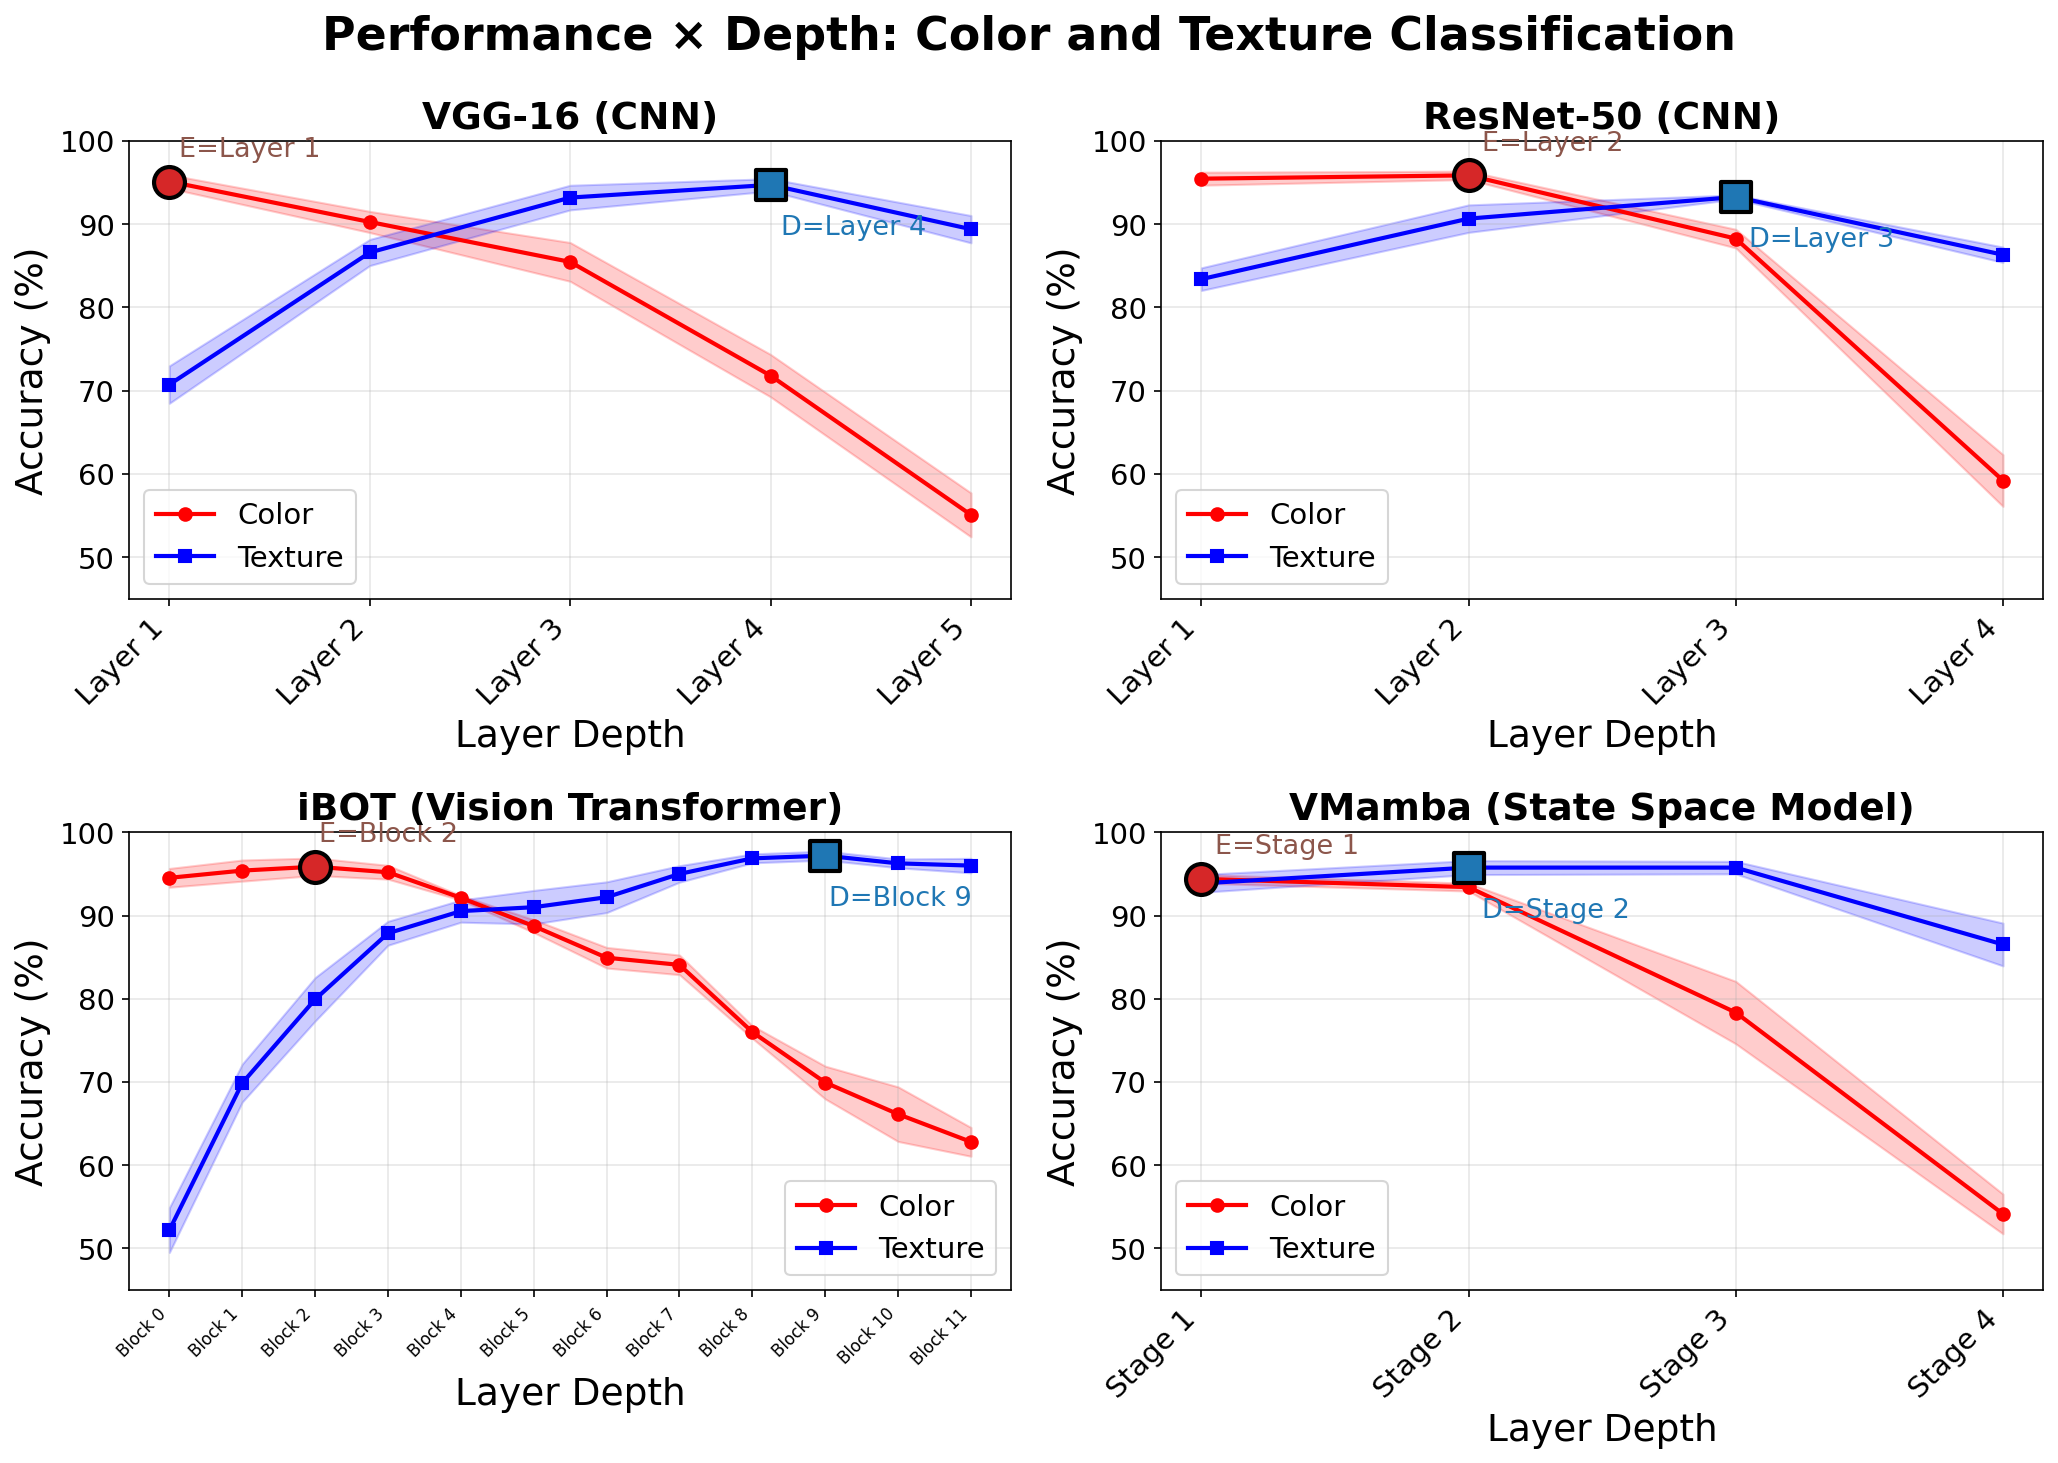
\includegraphics[width=0.48\textwidth]{curvas_desempenho_profundidade.png}}
\caption{Desempenho por profundidade: classificação de cor e textura para
         VGG-16, ResNet-50, iBOT e VMamba. Marcadores indicam as melhores
         camadas por atributo (E=cor, D=textura).}
\label{fig_depth}
\end{figure}

\subsection{Resultados da Fusão por Concatenação}

A Tabela~\ref{tab5} apresenta a configuração de fusão para cada backbone,
e as Tabelas~\ref{tab6} e~\ref{tab7} apresentam os resultados.

\begin{table}[htbp]
\caption{Configuração de fusão por backbone (Experimento~2).}
\begin{center}
\begin{tabular}{c|c|c|c|c|c}
\hline
\textbf{Backbone} & \textbf{E (cor)} & \textbf{Dim E}
                  & \textbf{D (tex.)} & \textbf{Dim D} & \textbf{Dim z} \\
\hline
VGG-16    & Cam. 1 & 64  & Cam. 4  & 512  & 576  \\
ResNet-50 & BR 2   & 512 & BR 3    & 1024 & 1536 \\
iBOT      & Bl. 2  & 384 & Bl. 9   & 384  & 768  \\
VMamba    & Est. 1 & 96  & Est. 2  & 192  & 288  \\
\hline
\end{tabular}
\label{tab5}
\end{center}
\end{table}

\begin{table}[htbp]
\caption{Resultados de fusão por concatenação — classificação de cor.}
\begin{center}
\begin{tabular}{c|c|c|c|c}
\hline
\textbf{Backbone} & \textbf{E (cor)} & \textbf{D (tex.)}
                  & \textbf{Z (fusão)} & \textbf{$\Delta$} \\
\hline
VGG-16    & \textbf{95,13\%} & 71,80\% & 86,13\% & $-$9,00\%  \\
ResNet-50 & \textbf{95,87\%} & 88,27\% & 94,13\% & $-$1,73\%  \\
iBOT      & \textbf{96,93\%} & 81,33\% & 85,13\% & $-$11,80\% \\
VMamba    & \textbf{94,80\%} & 93,93\% & 94,13\% & $-$0,67\%  \\
\hline
\end{tabular}
\label{tab6}
\end{center}
\end{table}

\begin{table}[htbp]
\caption{Resultados de fusão por concatenação — classificação de textura.}
\begin{center}
\begin{tabular}{c|c|c|c|c}
\hline
\textbf{Backbone} & \textbf{E (cor)} & \textbf{D (tex.)}
                  & \textbf{Z (fusão)} & \textbf{$\Delta$} \\
\hline
VGG-16    & 70,73\% & \textbf{94,73\%} & 94,73\% & $+$0,00\% \\
ResNet-50 & 90,67\% & 93,27\%          & \textbf{93,53\%} & $+$0,27\% \\
iBOT      & 78,33\% & \textbf{87,80\%} & 88,07\% & $+$0,27\% \\
VMamba    & 88,40\% & \textbf{94,33\%} & 93,40\% & $-$0,93\% \\
\hline
\end{tabular}
\label{tab7}
\end{center}
\end{table}

Os resultados de fusão mostram que a concatenação simples geralmente não
melhora o desempenho.
Para classificação de cor, a fusão degradou consistentemente a acurácia
comparada ao uso da camada especializada em cor~(E), com o iBOT
apresentando a maior degradação~($-$11,80\%).
Para textura, os resultados foram mistos, com melhorias mínimas para
ResNet-50 e iBOT~($+$0,27\%) e degradação para VMamba~($-$0,93\%).

\subsection{Resultados da Fusão Adaptativa com MoE}

A Tabela~\ref{tab_moe} apresenta os resultados do modelo MoE proposto.
Comparado ao Experimento~1 (melhor camada única) e ao Experimento~2
(concatenação), o MoE supera ambos em quase todas as combinações de
backbone e atributo.

\begin{table}[htbp]
\caption{Resultados do modelo MoE para classificação de cor e textura.}
\begin{center}
\begin{tabular}{c|c|c|c|c}
\hline
\textbf{Backbone} & \textbf{MoE Cor (\%)} & \textbf{Std}
                  & \textbf{MoE Tex. (\%)} & \textbf{Std} \\
\hline
VGG-16    & 93,40 & 0,71 & 96,13 & 1,00 \\
ResNet-50 & 97,27 & 0,71 & \textbf{97,67} & 0,47 \\
iBOT      & \textbf{97,33} & 0,56 & 95,47 & 0,96 \\
VMamba    & 96,93 & 1,02 & \textbf{98,00} & 0,73 \\
\hline
\end{tabular}
\label{tab_moe}
\end{center}
\end{table}

A Tabela~\ref{tab_comparacao} consolida a comparação entre os três
experimentos para as melhores configurações de cada backbone.

\begin{table}[htbp]
\caption{Comparação entre camada única (Exp.\,1), concatenação (Exp.\,2)
         e MoE (Exp.\,3). Valores em \%. $\Delta_1$: ganho sobre
         camada única; $\Delta_2$: ganho sobre concatenação.}
\begin{center}
\begin{tabular}{c|c|c|c|c|c|c}
\hline
\textbf{Config.} & \textbf{Exp.1} & \textbf{Exp.2}
                 & \textbf{MoE} & \textbf{$\Delta_1$}
                 & \textbf{$\Delta_2$} & \textbf{Melhor} \\
\hline
VGG Cor      & 95,13 & 86,13 & 93,40 & $-$1,73 & $+$7,27 & Exp.1 \\
VGG Tex.     & 94,73 & 94,73 & 96,13 & $+$1,40 & $+$1,40 & \textbf{MoE} \\
ResNet Cor   & 95,87 & 94,13 & 97,27 & $+$1,40 & $+$3,13 & \textbf{MoE} \\
ResNet Tex.  & 93,27 & 93,53 & 97,67 & $+$4,40 & $+$4,13 & \textbf{MoE} \\
iBOT Cor     & 95,87 & 85,13 & 97,33 & $+$1,46 & $+$12,20 & \textbf{MoE} \\
iBOT Tex.    & 97,20 & 88,07 & 95,47 & $-$1,73 & $+$7,40 & Exp.1 \\
VMamba Cor   & 94,41 & 94,13 & 96,93 & $+$2,52 & $+$2,80 & \textbf{MoE} \\
VMamba Tex.  & 95,76 & 93,40 & 98,00 & $+$2,24 & $+$4,60 & \textbf{MoE} \\
\hline
\end{tabular}
\label{tab_comparacao}
\end{center}
\end{table}

O MoE é o melhor método em 6 das 8 configurações avaliadas.
As duas exceções — VGG-16 cor e iBOT textura — correspondem a casos em que
uma única camada especializada já apresenta desempenho muito elevado
(95,13\% e 97,20\%, respectivamente), deixando pouco espaço para melhoria.
Notavelmente, o ganho do MoE sobre a concatenação é expressivo em todas as
configurações, com destaque para iBOT cor~($+$12,20~pp) e VMamba
textura~($+$4,60~pp).

\subsection{Avaliação CBIR: mAP@10, R@1 e R@5}

As Tabelas~\ref{tab_cbir_color} e~\ref{tab_cbir_texture} apresentam a
avaliação dos embeddings segundo o protocolo CBIR: para cada imagem de
consulta do conjunto de teste, todas as imagens de treino são ranqueadas
por distância euclidiana e as métricas são calculadas sobre os
$K\!=\!10$ mais próximos.
mAP@10 é a precisão média nos 10 vizinhos mais próximos; R@1 e R@5
indicam, respectivamente, a fração de consultas em que o resultado
correto aparece na primeira e entre as cinco primeiras posições.

\begin{table}[htbp]
\caption{Avaliação CBIR — Cor (\%). Melhor valor por backbone em
         \textbf{negrito}.}
\begin{center}
\begin{tabular}{c|l|c|c|c}
\hline
\textbf{Backbone} & \textbf{Método} & \textbf{mAP@10}
                  & \textbf{R@1} & \textbf{R@5} \\
\hline
\multirow{4}{*}{VGG-16}
  & Cam. Rasa (E)           & \textbf{94,47} & \textbf{95,47} & \textbf{99,13} \\
  & Cam. Prof. (D)          & 72,92 & 72,20 & 91,53 \\
  & Concat.                 & 83,89 & 86,53 & 96,73 \\
  & MoE \textit{(proposto)} & 93,71 & 94,93 & 98,07 \\
\hline
\multirow{4}{*}{ResNet-50}
  & Cam. Rasa (E)           & 94,51 & 96,13 & 99,00 \\
  & Cam. Prof. (D)          & 86,25 & 87,67 & 97,20 \\
  & Concat.                 & 92,40 & 93,93 & 98,33 \\
  & MoE \textit{(proposto)} & \textbf{96,09} & \textbf{96,07} & \textbf{98,67} \\
\hline
\multirow{4}{*}{iBOT}
  & Cam. Rasa (E)           & 94,93 & 95,40 & 99,13 \\
  & Cam. Prof. (D)          & 71,85 & 72,00 & 92,47 \\
  & Concat.                 & 75,06 & 76,67 & 94,13 \\
  & MoE \textit{(proposto)} & \textbf{97,96} & \textbf{98,27} & \textbf{99,47} \\
\hline
\multirow{4}{*}{VMamba}
  & Cam. Rasa (E)           & 93,20 & 94,33 & 98,47 \\
  & Cam. Prof. (D)          & 91,73 & 93,13 & 98,33 \\
  & Concat.                 & 92,51 & 93,67 & 98,40 \\
  & MoE \textit{(proposto)} & \textbf{96,91} & \textbf{96,87} & \textbf{99,07} \\
\hline
\end{tabular}
\label{tab_cbir_color}
\end{center}
\end{table}

\begin{table}[htbp]
\caption{Avaliação CBIR — Textura (\%). Melhor valor por backbone em
         \textbf{negrito}.}
\begin{center}
\begin{tabular}{c|l|c|c|c}
\hline
\textbf{Backbone} & \textbf{Método} & \textbf{mAP@10}
                  & \textbf{R@1} & \textbf{R@5} \\
\hline
\multirow{4}{*}{VGG-16}
  & Cam. Rasa (E)           & 70,87 & 70,33 & 91,27 \\
  & Cam. Prof. (D)          & 94,78 & 96,20 & \textbf{99,47} \\
  & Concat.                 & 94,53 & 96,13 & 99,27 \\
  & MoE \textit{(proposto)} & \textbf{95,98} & \textbf{96,80} & 99,07 \\
\hline
\multirow{4}{*}{ResNet-50}
  & Cam. Rasa (E)           & 90,35 & 90,80 & 99,07 \\
  & Cam. Prof. (D)          & 93,72 & 95,60 & 99,20 \\
  & Concat.                 & 93,05 & 94,47 & 98,87 \\
  & MoE \textit{(proposto)} & \textbf{97,88} & \textbf{98,13} & \textbf{99,20} \\
\hline
\multirow{4}{*}{iBOT}
  & Cam. Rasa (E)           & 78,90 & 79,33 & 94,33 \\
  & Cam. Prof. (D)          & \textbf{96,40} & \textbf{97,73} & \textbf{99,80} \\
  & Concat.                 & 96,30 & 97,67 & 99,73 \\
  & MoE \textit{(proposto)} & 95,10 & 95,40 & 98,53 \\
\hline
\multirow{4}{*}{VMamba}
  & Cam. Rasa (E)           & 87,66 & 88,80 & 97,33 \\
  & Cam. Prof. (D)          & 93,52 & 95,53 & 99,13 \\
  & Concat.                 & 93,05 & 95,07 & 99,13 \\
  & MoE \textit{(proposto)} & \textbf{97,89} & \textbf{98,27} & \textbf{99,33} \\
\hline
\end{tabular}
\label{tab_cbir_texture}
\end{center}
\end{table}

O MoE apresenta as melhores métricas CBIR em 3 dos 4 backbones para cor
e em 3 dos 4 para textura.
A exceção do iBOT em textura confirma o mesmo padrão observado na
acurácia: o Bloco~9 do iBOT gera representações de textura tão
discriminativas~(mAP@10 = 96,40\%) que o roteador tem dificuldade de
superá-las.
O ganho do MoE sobre a concatenação é expressivo em cor para o
iBOT~(+22,90~pp em mAP@10), confirmando que a fusão adaptativa resolve
o problema de degradação observado no Experimento~2.

% -----------------------------------------------------------------------
\section{DISCUSSÃO}

Os resultados experimentais deste estudo confirmam que o padrão de
sensibilidade por camada observado em CNNs clássicas se estende às
arquiteturas modernas baseadas em Vision Transformers e Modelos de Espaço
de Estados.
Em todos os backbones avaliados, as camadas iniciais capturam
consistentemente características mais adequadas para classificação de cor,
enquanto as camadas mais profundas são mais eficazes para o reconhecimento
de textura.

A acurácia excepcional do iBOT em textura~(97,20\%) sugere que o objetivo
de modelagem de imagem mascarada autossupervisionado incentiva o aprendizado
de representações estruturais ricas nas camadas profundas.

O Experimento~2 demonstrou que a concatenação simples não é uma estratégia
eficaz de fusão para tarefas de atributo específico.
A introdução do modelo MoE~(Experimento~3) resolve essa limitação ao
aprender dinamicamente os pesos de contribuição de cada camada.
O roteador treinável adapta-se ao conteúdo da imagem: imagens mais
discriminativas por cor induzem $\alpha$ alto; imagens mais discriminativas
por textura induzem $\beta$ alto.
Esse comportamento torna o MoE superior à concatenação em todas as
configurações avaliadas, e superior à camada única em 6 das 8 configurações.

A exceção do iBOT em textura~($-$1,73~pp sobre o Exp.1) é compreensível:
o Bloco~9 do iBOT já fornece representações de textura excepcionalmente
ricas~(97,20\%); o roteador não consegue melhorar o que já está próximo do
limite do conjunto.
Para a VGG-16 em cor, a assimetria entre a dimensão muito pequena da camada
rasa~(64d) e a camada profunda~(256d) pode limitar a capacidade do projetor
$h_E$.

Em termos práticos, o MoE oferece uma solução unificada para sistemas de
recuperação baseada em atributos visuais, eliminando a necessidade de
selecionar manualmente a camada mais adequada para cada tipo de consulta.

% -----------------------------------------------------------------------
\section{CONCLUSÃO}

Este trabalho apresentou uma avaliação abrangente da extração de
características por camada em múltiplas arquiteturas de aprendizado
profundo para classificação de cor e textura em imagens de moda, e propôs
um modelo de fusão adaptativa baseado em Mixture of Experts~(MoE).

Os Experimentos~1 e~2 confirmam que o padrão de sensibilidade por camada
se generaliza de CNNs clássicas para Vision Transformers e Modelos de
Espaço de Estados, e que a concatenação simples não é uma estratégia
eficaz de fusão.
O Experimento~3 introduz o MoE como uma solução que aprende
adaptativamente os pesos das representações rasa~(cor) e
profunda~(textura), superando tanto as representações de camada única
quanto a fusão por concatenação em 6 das 8 configurações avaliadas.
Os melhores resultados com MoE foram: 98,00\%~(VMamba, textura) e
97,33\%~(iBOT, cor).

Estes resultados têm implicações práticas para sistemas de recuperação de
imagens: o MoE oferece um único vetor de representação que se adapta ao
conteúdo da imagem, sem necessidade de seleção manual da camada.
Trabalhos futuros investigarão estratégias de roteamento com mais de dois
especialistas, a incorporação de atenção cruzada entre camadas, e a
extensão para tarefas de recuperação em larga escala.

% -----------------------------------------------------------------------
\section*{AGRADECIMENTOS}

Este trabalho foi apoiado pelo Conselho Nacional de Desenvolvimento
Científico e Tecnológico~(CNPq, Brasil).

% -----------------------------------------------------------------------
\begin{thebibliography}{00}

\bibitem{b1}
S. R. Dubey, ``A decade survey of content based image retrieval using deep
learning,'' \emph{IEEE Trans. Circuits Syst. Video Technol.}, vol.~32,
no.~5, pp.~2687--2704, 2021.

\bibitem{b2}
A. Baloian, N. Murrugarra-Llerena, and J. M. Saavedra, ``Scalable visual
attribute extraction through hidden layers of a residual convnet,''
\emph{arXiv preprint arXiv:2104.00161}, 2021.

\bibitem{b3}
J. Deng, W. Dong, R. Socher, L.-J. Li, K. Li, and L. Fei-Fei,
``ImageNet: A large-scale hierarchical image database,'' in
\emph{Proc. IEEE CVPR}, 2009, pp.~248--255.

\bibitem{b4}
K. He, X. Zhang, S. Ren, and J. Sun, ``Deep residual learning for image
recognition,'' in \emph{Proc. IEEE CVPR}, 2016, pp.~770--778.

\bibitem{b7}
K. Simonyan and A. Zisserman, ``Very deep convolutional networks for
large-scale image recognition,'' \emph{arXiv preprint arXiv:1409.1556},
2014.

\bibitem{b8}
M. Moresco, A. D. S. Britto, Y. M. Costa, L. J. Senger, and
A. G. Hochuli, ``Combining multi-layer features for plant species
classification in a Siamese network,'' in \emph{Proc. IEEE SMC}, 2022,
pp.~2446--2451.

\bibitem{b9}
V. M. Araújo, A. S. Britto Jr., L. S. Oliveira, and A. L. Koerich,
``Two-view fine-grained classification of plant species,''
\emph{Neurocomputing}, vol.~467, pp.~427--441, 2022.

\bibitem{b10}
K. Liang, H. Chang, S. Shan, and X. Chen, ``A unified multiplicative
framework for attribute learning,'' in \emph{Proc. IEEE ICCV}, 2015,
pp.~2506--2514.

\bibitem{b11}
C. Gan, T. Yang, and B. Gong, ``Learning attributes equals multi-source
domain generalization,'' in \emph{Proc. IEEE CVPR}, 2016, pp.~87--97.

\bibitem{b12}
S. M. Youssef, ``ICTEDCT-CBIR: Integrating curvelet transform with
enhanced dominant colors extraction and texture analysis for efficient
content-based image retrieval,'' \emph{Comput. Electr. Eng.}, vol.~38,
no.~5, pp.~1358--1376, 2012.

\bibitem{b13}
A. Irtaza, M. A. Jaffar, E. Aleisa, and T. S. Choi, ``Embedding neural
networks for semantic association in content based image retrieval,''
\emph{Multimedia Tools Appl.}, vol.~72, pp.~1911--1931, 2014.

\bibitem{b14}
H. F. Atlam, G. Attiya, and N. El-Fishawy, ``Integration of color and
texture features in CBIR system,'' \emph{Int. J. Comput. Appl.},
vol.~164, no.~3, pp.~23--29, 2017.

\bibitem{b15}
C. H. Lin, R. T. Chen, and Y. K. Chan, ``A smart content-based image
retrieval system based on color and texture feature,'' \emph{Image Vis.
Comput.}, vol.~27, no.~6, pp.~658--665, 2009.

\bibitem{b16}
A. Gu and T. Dao, ``Mamba: Linear-time sequence modeling with selective
state spaces,'' \emph{arXiv preprint arXiv:2312.00752}, 2023.

\bibitem{b17}
J. Zhou et al., ``iBOT: Image BERT pre-training with online tokenizer,''
\emph{arXiv preprint arXiv:2111.07832}, 2021.

\bibitem{b23}
D. Mukherjee, R. Mondal, P. K. Singh, R. Sarkar, and D. Bhattacharjee,
``EnsembleNet: A hybrid approach for vehicle detection and traffic density
estimation based on Faster R-CNN and YOLO,'' \emph{Neural Comput. Appl.},
vol.~32, no.~15, pp.~14207--14228, 2020.

\bibitem{b24}
J. Yue, Z. Li, L. Liu, and Z. Fu, ``Content-based image retrieval using
color and texture,'' in \emph{Proc. ICIG}, 2011, pp.~833--837.

\bibitem{b25}
E. Prakasa, ``Texture feature extraction by using local binary pattern,''
\emph{INKOM J.}, vol.~1, no.~1, pp.~1--6, 2016.

\bibitem{b26}
J. Long, E. Shelhamer, and T. Darrell, ``Fully convolutional networks for
semantic segmentation,'' in \emph{Proc. IEEE CVPR}, 2015, pp.~3431--3440.

\bibitem{b27}
Y. Guo, Y. Liu, T. Georgiou, and M. S. Lew, ``A review of semantic
segmentation using deep neural networks,'' \emph{Int. J. Multimedia Inf.
Retr.}, vol.~7, no.~2, pp.~87--93, 2018.

\bibitem{b28}
J. de Matos, L. E. S. de Oliveira, A. D. S. Britto Jr., and
A. L. Koerich, ``Large-margin representation learning for texture
classification,'' \emph{Pattern Recognit. Lett.}, vol.~170, pp.~39--47,
2023.

\bibitem{bzeiler}
M. D. Zeiler and R. Fergus, ``Visualizing and understanding convolutional
networks,'' in \emph{Proc. ECCV}, 2014, pp.~818--833.

\bibitem{bkazami}
H. Kazami, N. Touvron, M. Cord, and P. Perez, ``What do vision
transformers learn? A visual exploration,''
\emph{arXiv preprint arXiv:2212.06727}, 2022.

\bibitem{bmoe_orig}
R. A. Jacobs, M. I. Jordan, S. J. Nowlan, and G. E. Hinton,
``Adaptive mixtures of local experts,''
\emph{Neural Computation}, vol.~3, no.~1, pp.~79--87, 1991.

\bibitem{bmoe_cao}
Z. Cao et al., ``Multi-modal gated mixture of local-to-global experts for
dynamic image fusion,'' in \emph{Proc. IEEE/CVF ICCV}, 2023,
pp.~23555--23564.

\end{thebibliography}

\end{document}
